\documentclass[a4paper,11pt]{article}

\usepackage[margin=2.5cm]{geometry}
\usepackage{amsmath,amssymb}
\usepackage{booktabs}
\usepackage{graphicx}
\usepackage{caption}
\usepackage{setspace}

\newcommand{\sfincs}{\textsc{SFINCS}}
\newcommand{\hecras}{\textsc{HEC-RAS}}

\doublespacing

\setcounter{figure}{0}
\setcounter{table}{0}
\renewcommand{\thefigure}{S\arabic{figure}}
\renewcommand{\thetable}{S\arabic{table}}

\begin{document}

\begin{center}
{\Large Supplementary Material}

\vspace{0.5em}
{\large Supplementary material for:}

\vspace{0.3em}
{\large From roughness uncertainty to model-structure effects in 2D flood inundation models: a Monte Carlo comparison of SFINCS and HEC-RAS}

\vspace{0.5em}
Salvador Navas, \'Alvaro Gal\'an, Manuel del Jesus
\end{center}

\paragraph{Robustness of main conclusions to inter-class Manning correlation.}
The following figures and tables document the Gaussian copula
importance-sampling procedure and its results in full, supporting the
correlated-roughness robustness analysis reported in the main manuscript.

\begin{figure}[!ht]
  \centering
  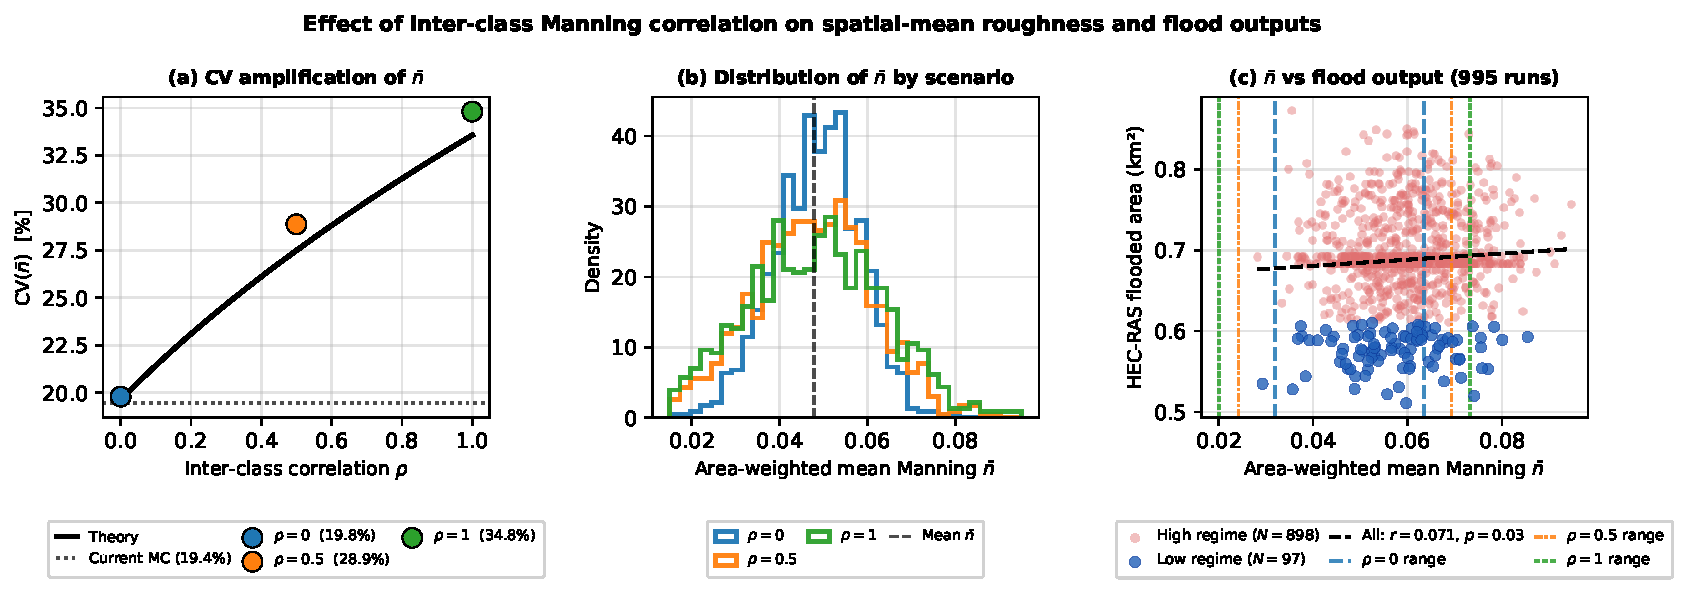
\includegraphics[width=\textwidth]{figures/fig_copula_analysis.pdf}
  \caption{Effect of inter-class Manning correlation on spatial-mean roughness
    and flood outputs ($N = 1\,000$ Gaussian copula samples per scenario).
    (a)~Theoretical CV amplification of the area-weighted mean Manning
    $\bar{n}$ with equi-correlation $\rho$ (solid curve); markers show
    empirical values; dotted line marks the reference independent-MC ensemble.
    (b)~Step histograms of $\bar{n}$: the distribution widens from
    CV\,=\,19.8\% ($\rho=0$) to 34.8\% ($\rho=1$) with no shift in the mean
    ($\bar{n}\approx 0.048$~m$^{-1/3}$s).
    (c)~$\bar{n}$ against HEC-RAS flooded area for 995 valid simulations
    coloured by hydraulic regime (upper-left legend: 5th--95th percentile
    range of $\bar{n}$ per scenario; lower-right legend: regime counts and
    regression); $r=0.071$ ($p=0.03$, $r^2<0.01$) shows only a weak direct
    association between inter-class Manning correlation and domain-scale
    flooded area; the regime fractions under correlated sampling are
    quantified in Supplementary Figure~S3.}
  \label{fig:copula}
\end{figure}

\begin{figure}[!ht]
  \centering
  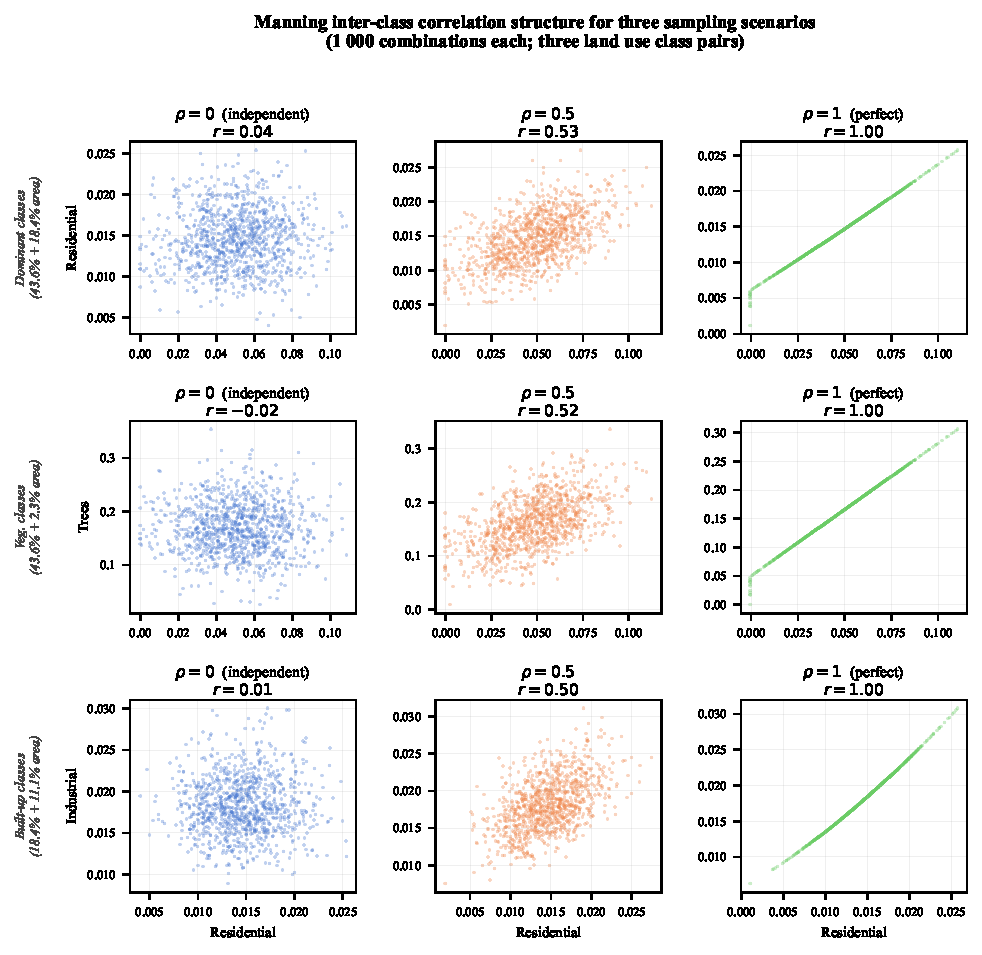
\includegraphics[width=\textwidth]{figures/fig_copula_scatter.pdf}
  \caption{Pairwise scatter plots of Manning $n$ values for three representative
    land use class pairs and three correlation scenarios
    ($N = 1\,000$ Gaussian copula samples each).
    Rows correspond to class pairs (dominant: sparse vegetation + residential;
    vegetation: sparse vegetation + trees; built-up: residential + industrial);
    columns correspond to equi-correlation values
    $\rho \in \{0,\,0.5,\,1.0\}$.
    Empirical Pearson $r$ confirms the copula reproduces the prescribed
    dependence structure.}
  \label{fig:copula_scatter}
\end{figure}

\begin{figure}[!ht]
  \centering
  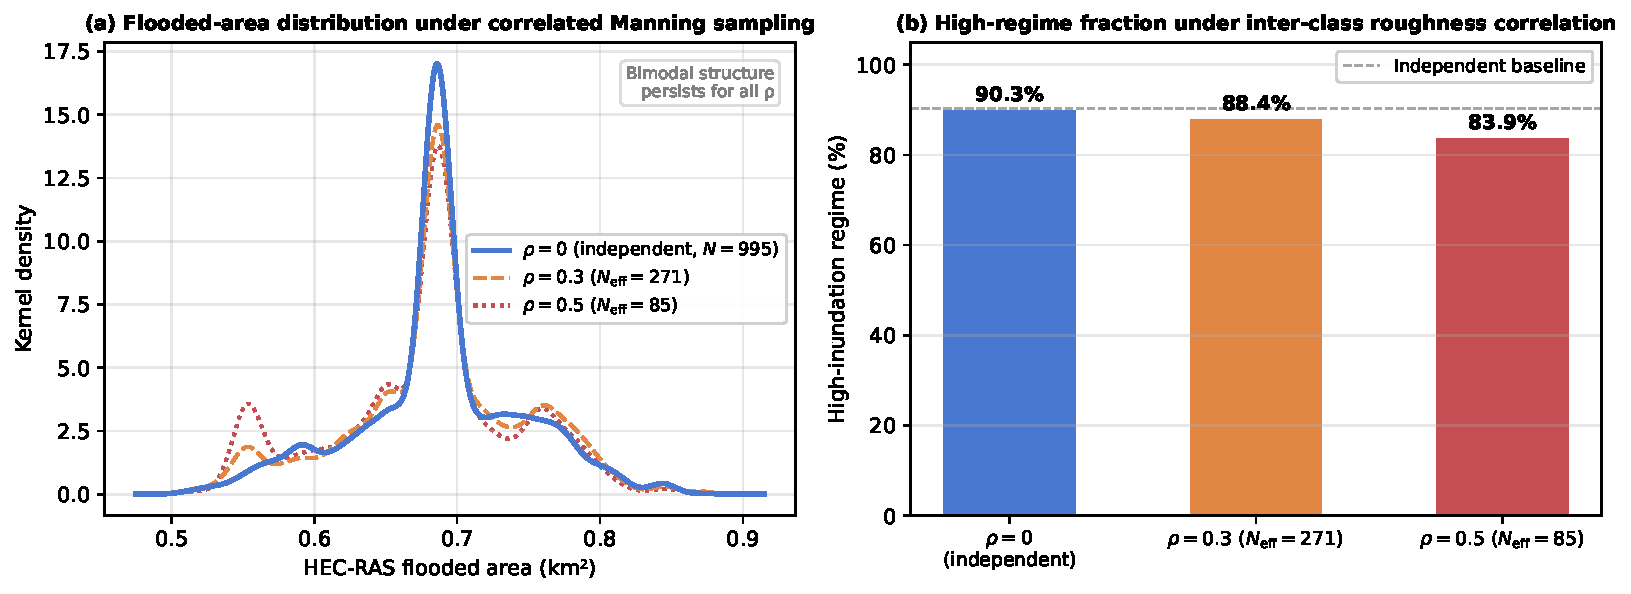
\includegraphics[width=\textwidth]{figures/fig_copula_is.pdf}
  \caption{Importance-sampling robustness check for inter-class Manning correlation.
    (\textbf{a})~Weighted kernel density estimates of \hecras{} flooded area
    under independent sampling ($\rho = 0$, $N = 995$) and two correlated
    scenarios ($\rho = 0.3$, effective $N = 271$; $\rho = 0.5$, effective $N = 85$).
    Weights are the ratio of the equicorrelation Gaussian copula density to
    the independent sampling density, computed from empirical probability
    integral transforms of the 9-class Manning vector.
    The bimodal structure of the \hecras{} response is preserved for all
    values of~$\rho$ shown.
    (\textbf{b})~High-inundation-regime fraction (weighted percentage) as a
    function of equicorrelation~$\rho$.
    The fraction decreases from 90.3\% (independent) to 88.4\% ($\rho = 0.3$)
    and 83.9\% ($\rho = 0.5$), confirming that the bimodal response is robust
    to plausible levels of inter-class roughness correlation.}
  \label{fig:copula_is}
\end{figure}

\begin{figure}[!ht]
  \centering
  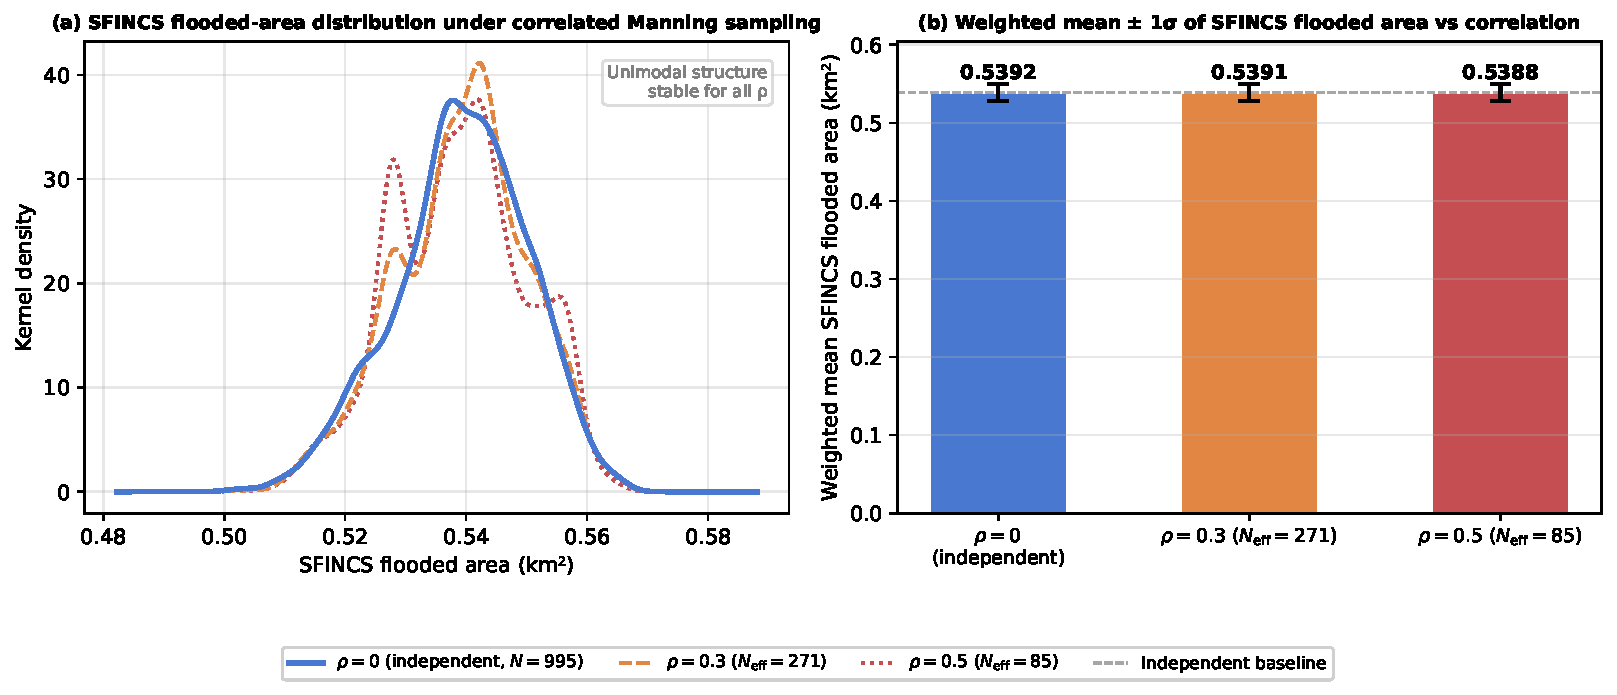
\includegraphics[width=\textwidth]{figures/fig_copula_is_sfincs.pdf}
  \caption{Importance-sampling robustness check for \sfincs{} under inter-class
    Manning correlation (counterpart to Supplementary Figure~S3 for \hecras{}).
    (\textbf{a})~Weighted kernel density estimates of \sfincs{} flooded area
    under independent sampling ($\rho = 0$, $N = 995$) and two correlated
    scenarios ($\rho = 0.3$, effective $N = 271$; $\rho = 0.5$, effective $N = 85$).
    The unimodal distribution is virtually unchanged across all values of~$\rho$.
    (\textbf{b})~Weighted mean $\pm1\sigma$ of \sfincs{} flooded area as a
    function of equicorrelation~$\rho$.
    The mean shifts by less than 0.1\% between $\rho = 0$ (0.5392~km$^2$) and
    $\rho = 0.5$ (0.5388~km$^2$), confirming that the unimodal \sfincs{}
    response is robust to plausible levels of inter-class roughness correlation.}
  \label{fig:copula_is_sfincs}
\end{figure}

\clearpage
\begin{table}[htbp]
  \centering
  \caption{Area-weighted spatial mean Manning $\bar{n}$ statistics under
    independent and Gaussian-copula correlated sampling
    ($N = 1\,000$ draws per scenario; domain area 1\,086~ha).
    P$_5$ and P$_{95}$ denote the 5th and 95th percentiles.}
  \label{tab:copula}
  \begin{tabular}{lcccccc}
    \hline
    Scenario & $\rho$ & Mean $\bar{n}$ & CV(\%) & P$_5$ & P$_{95}$ & P$_{95}$/P$_5$ \\
    \hline
    Independent (reference) & 0   & 0.0484 & 19.4 & 0.033 & 0.064 & 1.94 \\
    Copula $\rho = 0$        & 0   & 0.0486 & 19.8 & 0.032 & 0.063 & 1.98 \\
    Copula $\rho = 0.5$      & 0.5 & 0.0474 & 28.9 & 0.024 & 0.069 & 2.87 \\
    Copula $\rho = 1.0$      & 1.0 & 0.0474 & 34.8 & 0.020 & 0.073 & 3.66 \\
    \hline
  \end{tabular}
\end{table}

\bigskip
\begin{table}[htbp]
  \centering
  \caption{\textbf{Simulations removed prior to analysis} ($N = 5$, 0.5\% of 1\,000).
    Anomalies were detected using a robust $z$-score with threshold
    $k = 5$.
    Model: S\,=\,SFINCS; H\,=\,HEC-RAS.
    Four of the five anomalies were flagged in HEC-RAS; the SFINCS outputs
    for those four simulations lie within the normal ensemble range.
    Simulation~633 is the exception: the flagged anomaly originates in
    SFINCS (flooded area $= 0.467$~km$^2$), while the paired HEC-RAS
    output falls within the normal ensemble range.
    Ensemble medians for reference: HEC-RAS area $\approx 0.668$~km$^2$,
    depth $\approx 1.22$~m; SFINCS area $\approx 0.537$~km$^2$,
    depth $\approx 1.04$~m.}
  \label{tab:anomalous}
  \resizebox{\textwidth}{!}{%
  \begin{tabular}{cclp{2.4cm}ccccc}
    \toprule
    Sim. & Model & Flagged metric & Flagged value & $|z|_{\mathrm{robust}}$ &
    \multicolumn{2}{c}{HEC-RAS output} & \multicolumn{2}{c}{SFINCS output} \\
    \cmidrule(lr){6-7}\cmidrule(lr){8-9}
    & & & & & Area (km$^2$) & Depth (m) & Area (km$^2$) & Depth (m) \\
    \midrule
    29  & H & Mean depth   & 1.930~m        & 6.70 & 2.187 & 1.930 & 0.498 & 0.949 \\
    295 & H & Mean depth   & 1.772~m        & 5.21 & 1.664 & 1.772 & 0.499 & 0.948 \\
    633 & S & Flooded area & 0.467~km$^{2}$ & 6.84 & 0.865 & 1.545 & 0.467 & 1.005 \\
    724 & H & Mean depth   & 1.805~m        & 5.52 & 1.118 & 1.805 & 0.512 & 0.994 \\
    755 & H & Mean depth   & 1.834~m        & 5.79 & 1.865 & 1.834 & 0.503 & 0.962 \\
    \bottomrule
  \end{tabular}}
\end{table}

\end{document}
